\chapter{The Discovery of the Gluon}

In order to organize the vast amount of particles that have been discovered up to 1961 Murray Gell-Mann and Yuval Ne'eman proposed independently from each other the Eightfold Way.
The Eightfold Way organizes hadrons in dependence on the quantum variables strangeness and isospin. 
Mesons with a spin parity configuration of $0^-$ and baryons with a spin parity configuration of $\sfrac 12^+$ can both be organized in an octet.
Baryons with a spin parity configuration can be organized in a decuplet of which the tenth particle, the $\Omega^-(sss)$ has been proposed theoretically before it has been experimentally found later \cite{Fritzsch2018}.
The early quark model was proposed by Gell-Mann and George Zweig in 1964 which consisted of only the up-, down- and strange-quark.
An electron-proton scattering event from 1968 revealed partons that took up half of the carried momentum and were thus the first indication of gluons \cite{Venker}.
A theoretical description is given by Quantum Chromodynamics (QCD) after which the baryon wave function must be antisymmetric thus leading to the introduction of colour as another quantum variable that can be either red, green or blue.
QCD is a $\text{SU}(3)$ gauge symmetry theory that describes the strong interaction.
It predicts eight gluons as a gauge boson that can interact with itself.
Particles with a colour charge can never be detected as a single particle, because the energy to separate two particles increases until a particle-antiparticle pair is produced
Due to confinement, quarks and gluons combine with other colour-carrying particles forming new hadrons in a process called hadronisation.
These hadrons can in turn form new hadrons themselves building a cascade of particles called a jet.
The first evidence for jets was observed at the Stanford Positron Electron Asymmetric Rings (SPEAR) at $\SI{7.4}{\giga\eV}$ in 1975.
In the year of 1979, all quarks except the top quark were found in experiments with the most recent discovery being the bottom quark in 1977.
However, there has been no experimental evidence for gluons so far.
One way to prove the existence of the gluon was via three-jet events as suggested by John Ellis.
Due to corrections at high energies, an electron-positron collision can produce a quark-antiquark pair with an additional gluon.
The emission of the gluon can be seen as the equivalent of bremsstrahlung in QCD resulting in a three-jet emission from each of the produced particles which are all in one plane due to momentum conservation.
Figure \ref{fig:jets} shows a schematic image of a two-jet and a three-jet configuration emission.
\begin{figure}
    \centering
    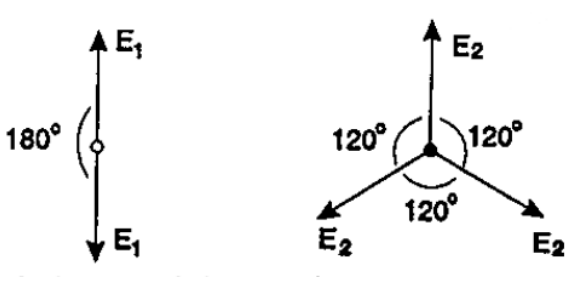
\includegraphics[width=0.4\textwidth]{figs/jets.png}
    \caption{Schematic image of a two-jet and a three-jet configuration \cite{Soding:1996zk}.}
    \label{fig:jets}
\end{figure}
The transition between a two and a three-jet event is continuous as the jets get broader the higher the energy gets until they can split up into three distinct jets.
A two jet-event starts at energies of $\SI{7.4}{\giga\eV}$ and turns into a three-jet event at around $\SI{20}{\giga\eV}$.
The experiment that managed to find the gluon was the Two Arm Spectrometer Solenoid (TASSO) at the Positron-Electron Tandem Ring Accelerator (PETRA) which is part of the Deutsches Elektronen-Synchrotron (DESY).
It started building in 1976 and was finished just two years later with a ring accelerator with a circumference of $\SI{2.304}{\kilo\meter}$ which could reach $\SI{27}{\giga\eV}$.
A schematic picture of TASSO is shown in figure \ref{fig:TASSO}.
\begin{figure}
    \centering
    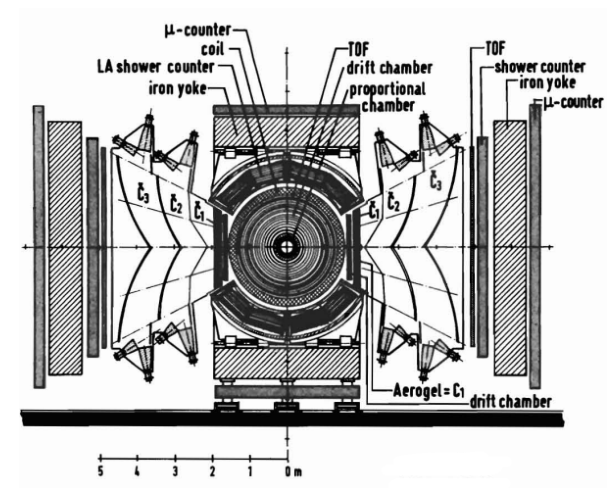
\includegraphics[width=0.4\textwidth]{figs/TASSO.png}
    \caption{Schematic image the TASSO-detector \cite{TASSO:1979xej}.}
    \label{fig:TASSO}
\end{figure}
The detector had two hadron-identifying arms, an aerogel and two gas cherenkov detectors and a time-of-flight and shower counters.
Its main use was the search for the three-jet event in one plane.
The first three-jet event was detected in 1979 at a center of mass energy of $\SI{27.4}{\giga\eV}$.
When comparing the experimental results to the theory, the problem occurred that perturbation theory is not useable for low energies which led to the introduction of event shape variables.
The event shape variables could be used to distinguish between different QCD models, one in which there are no gluons and one in which there are.
The experimental results were in good agreement with the prediction of a model with gluon, as can be seen in figure \ref{fig:GluonResultsA} that shows different predictions for a model without gluons resembled by the dashed line and a model with gluons \cite{Branson:1994eu}.
\begin{figure}
    \centering
    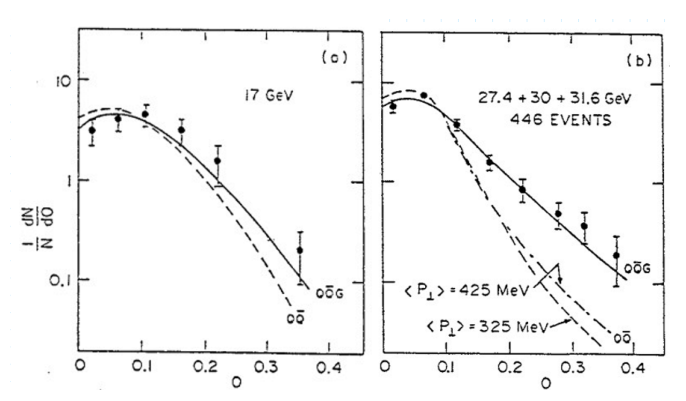
\includegraphics[width=0.4\textwidth]{figs/gluonResultsA.png}
    \caption{Experimental results comparing a QCD model with gluons and with a QCD model without gluons with data from TASSO \cite{Branson:1994eu}.}
    \label{fig:GluonResultsA}
\end{figure}
By measuring the angle in a Lorentz-boosted center-of-momentum frame, called the Ellis-Karliner angle, it is possible to analyse the spin of the gluon.
The Ellis-Karliner angle distribution from TASSO is shown in figure \ref{fig:GluonResultsB} in which the experimental data matches the theoretical prediction of a vector particle proving that the gluon has a spin of 1 \cite{Venker, Soding:1996zk}.
\begin{figure}
    \centering
    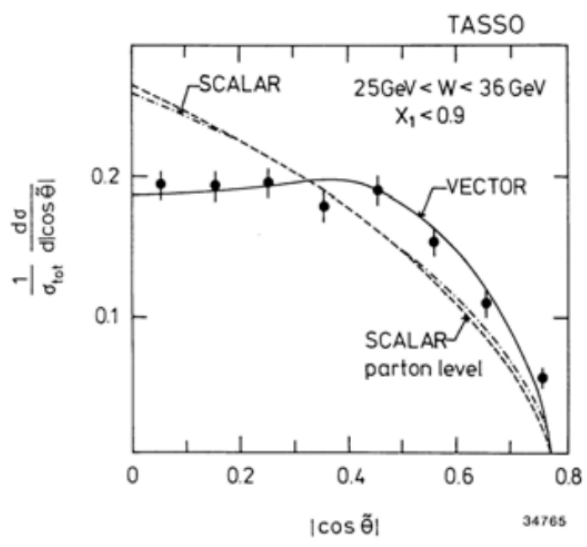
\includegraphics[width=0.4\textwidth]{figs/gluonResultsB.png}
    \caption{Ellis-Karliner angle distribution from TASSO \cite{Venker, Soding:1996zk}.}
    \label{fig:GluonResultsB}
\end{figure}
The discovery of the gluon is the perfect example of theory and experiments working together to discover new parts of physics as the gluon was originally predicted by QCD as a vector boson that could be emitted in three-jet events and was discovered in such an event with the exact characteristics it was predicted to have.